\section{Reconstrução de FEN e Detecção de Jogadas}
\label{sec:fen-jogadas}

Com um \texttt{piece\_map} completo (casa $\to$ tipo e cor da peça), obtido combinando a
ocupação clássica, a cor clássica e o tipo previsto pela ResNet-34, a posição pode ser
serializada em \textbf{FEN} (\textit{Forsyth-Edwards Notation}), a notação padrão para
posições de xadrez.

\subsection{FEN completa --- seis campos}

A função \texttt{board\_to\_fen} produz uma FEN \textbf{completa}: o campo de
posicionamento de peças é lido diretamente do tabuleiro (fileira 8 $\to$ 1, maiúsculas
para peças brancas, casas vazias colapsadas em contagens), enquanto os outros cinco
campos --- lado a mover, direitos de roque, alvo de \textit{en passant}, contador de
meio-lances e número da jogada --- são fornecidos explicitamente e validados, pois não
podem ser inferidos a partir de uma única fotografia estática. A função
\texttt{castling\_rights\_from\_position} produz uma estimativa de melhor esforço dos
direitos de roque a partir de onde reis e torres estão posicionados (rei e torre nas
casas de origem $\Rightarrow$ direito de roque presumido).

\subsection{Ambiguidade de orientação de $180\degree$}

Ao ler uma imagem de forma totalmente automática (sem gabarito), a orientação do
tabuleiro é obtida a partir da densidade de bordas por linha/coluna
(\texttt{detect\_board\_rotation}). Essa heurística fixa corretamente o \textbf{eixo} do
tabuleiro (0\% de erro de eixo medido sobre 60 imagens), mas não resolve a ambiguidade de
$180\degree$: como as cores das casas de um tabuleiro de xadrez são simétricas sob
rotação de $180\degree$, não há, a partir de uma única imagem, informação suficiente
para decidir entre as duas orientações --- cerca de \textbf{42\%} dos tabuleiros ficam
efetivamente invertidos nessa leitura totalmente automática.

Isso não é tratado como um defeito a ser corrigido, mas como um \textbf{limite
intrínseco de uma imagem única}, documentado explicitamente: a função
\texttt{rotate\_piece\_map\_180} gera o mapa de peças da orientação alternativa, e o
sistema reporta \textbf{as duas FENs candidatas} --- o tabuleiro real é necessariamente
uma delas. Resolver a ambiguidade remanescente exigiria informação externa à imagem
(OCR dos rótulos de fileira/coluna do próprio tabuleiro físico, ou contexto de uma
partida em andamento), nenhuma das quais confiável neste dataset de imagens isoladas.

\subsection{Detecção de jogadas}

A comparação temporal entre dois mapas de ocupação booleanos identifica as casas que
mudaram de estado:

\begin{lstlisting}[language=Python]
def detect_moves(occ_a, occ_b):
    emptied  = occ_a & ~occ_b   # estava ocupada, agora vazia
    occupied = ~occ_a & occ_b   # estava vazia, agora ocupada
    return list(...)            # lista de (linha, coluna, tipo_de_mudanca)
\end{lstlisting}

Para uma jogada simples, espera-se exatamente 1 casa esvaziada e 1 casa ocupada; uma
captura resulta em 1 casa esvaziada e 0 ou 1 casa ocupada, dependendo de qual lado
capturou. A função \texttt{classify\_move} vai além do diff de ocupação: comparando dois
\texttt{piece\_map}s completos (antes/depois), ela infere o lance em notação UCI e uma
descrição textual, cobrindo os casos especiais do xadrez:

\begin{itemize}[nosep]
  \item \textbf{Lance simples} (ex.: \texttt{1.e4});
  \item \textbf{Captura} (ex.: \texttt{exd5});
  \item \textbf{Roque}, curto ou longo (ex.: \texttt{O-O}) --- identificado pelo padrão
        característico de movimentação simultânea de rei e torre;
  \item \textbf{\textit{En passant}} --- identificado quando um peão captura
        lateralmente sem que a casa capturada coincida com a casa de destino;
  \item \textbf{Promoção} (ex.: \texttt{e8=Q}) --- identificada quando um peão chega à
        última fileira e a peça na casa de destino muda de tipo.
\end{itemize}

Como o dataset não contém sequências de jogo reais (cada imagem é uma posição
independente), a lógica de \texttt{classify\_move} foi validada com posições
\textbf{controladas} --- montadas manualmente para cobrir cada caso especial --- e,
adicionalmente, aplicada a pares de imagens não relacionadas do dataset apenas para
demonstrar o comportamento da função (sem uma jogada real de referência para comparar).

\begin{figure}[H]
  \centering
  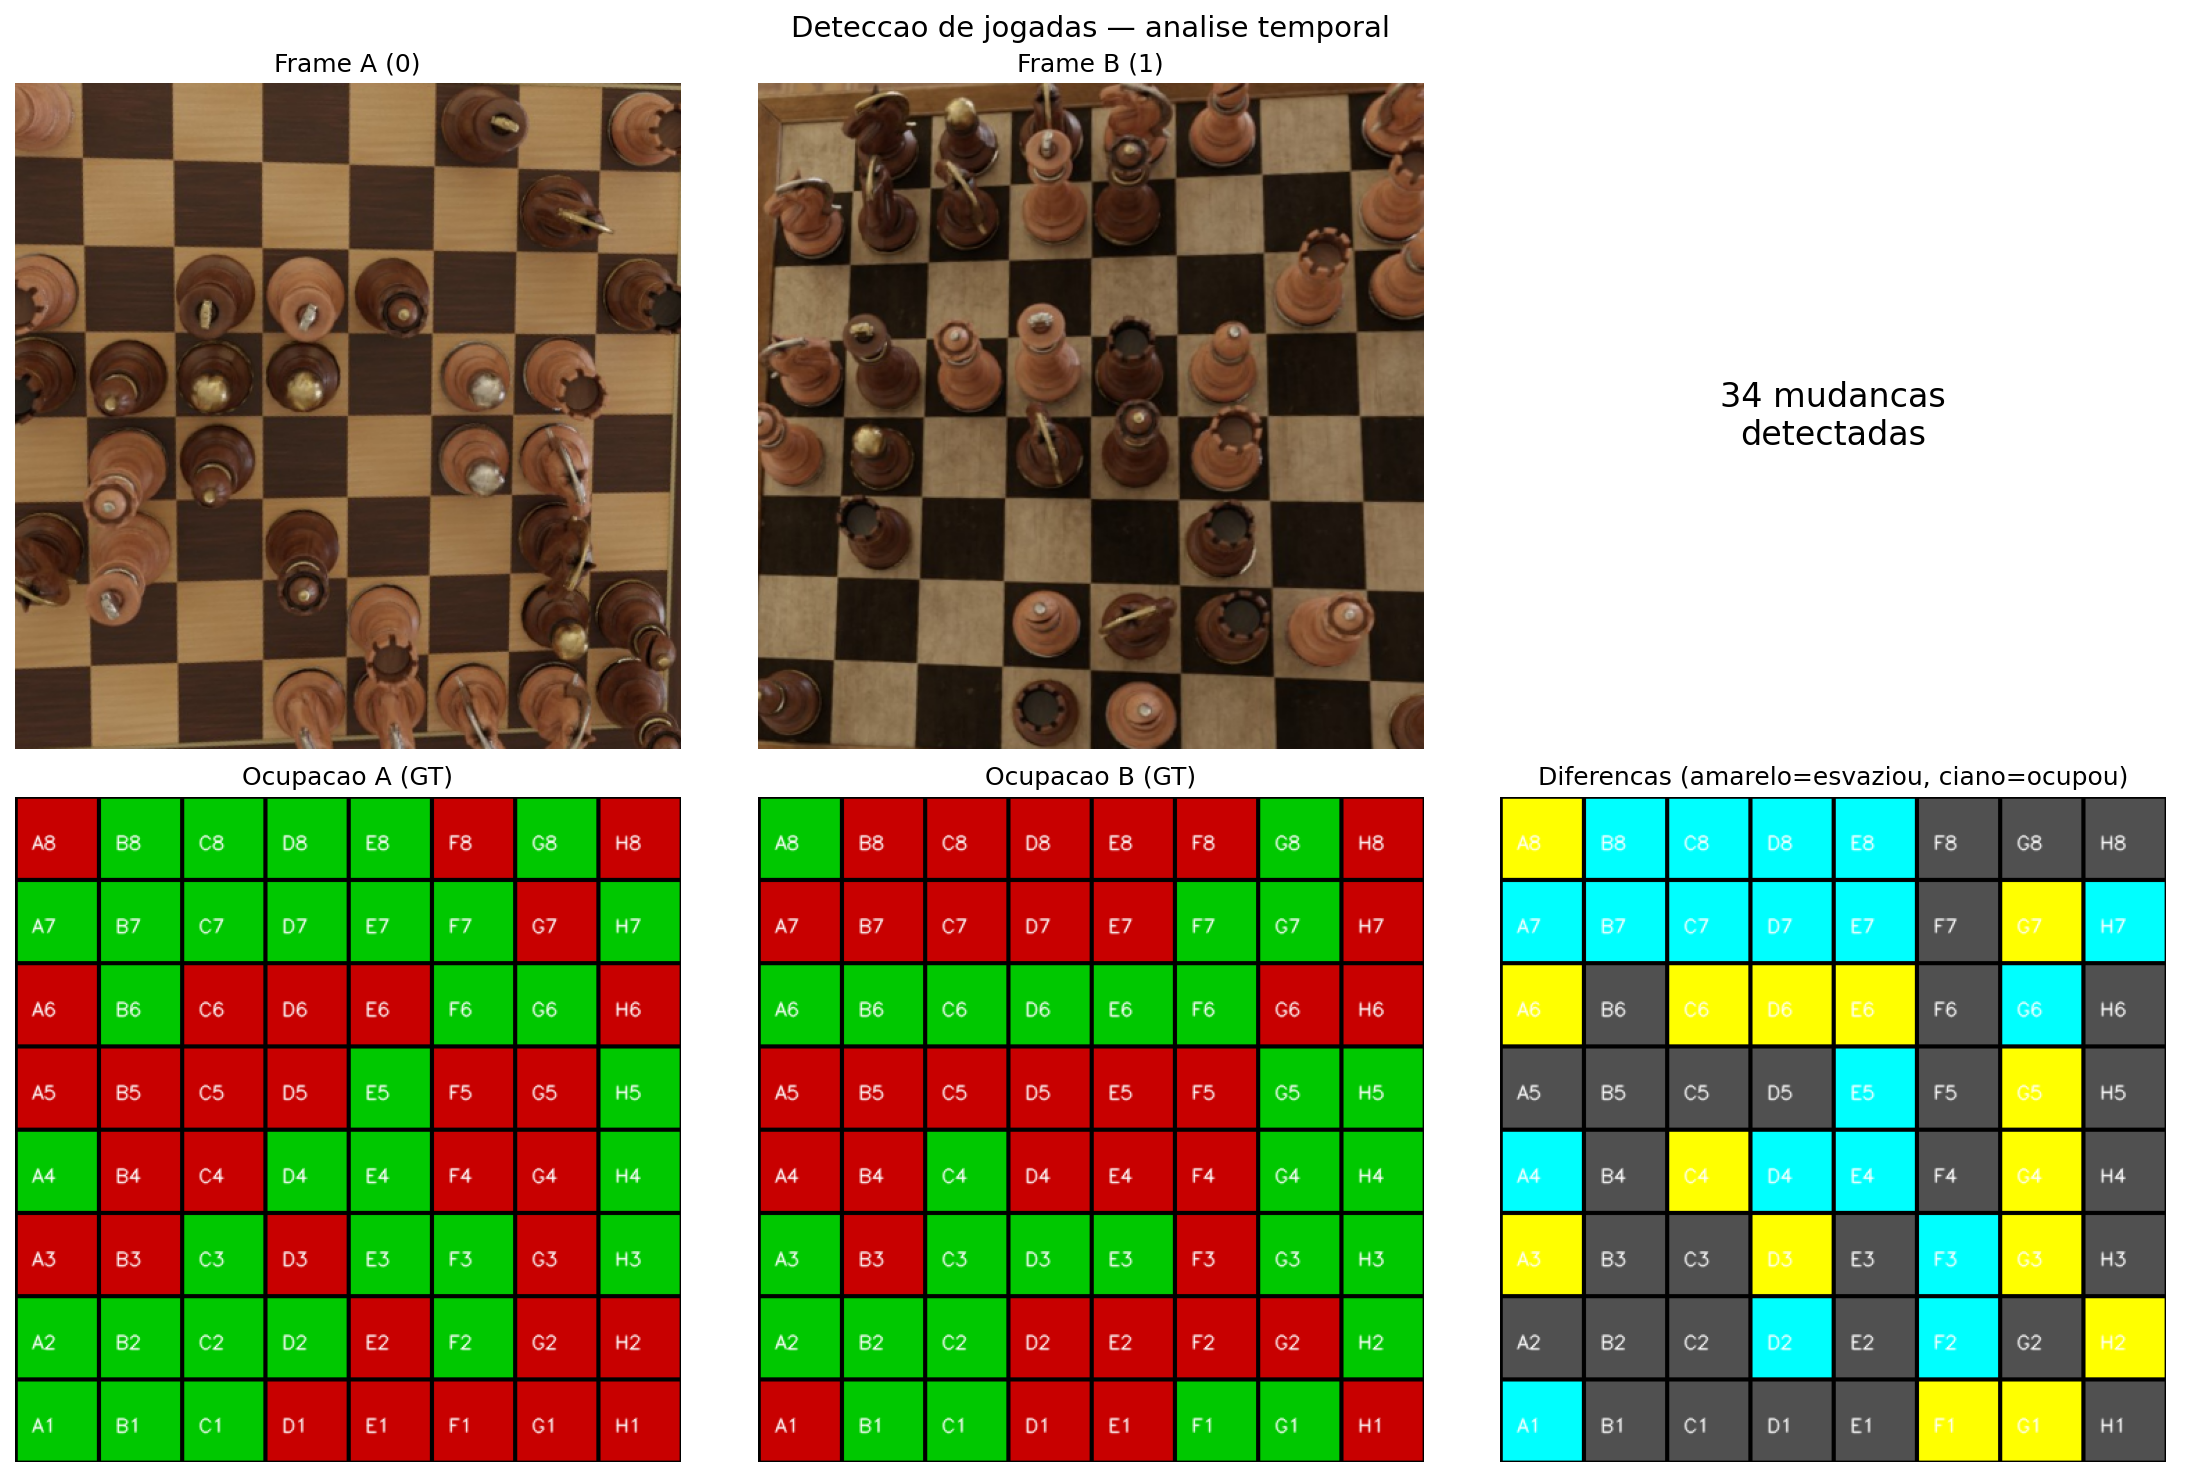
\includegraphics[width=0.85\textwidth]{../../intro/images/12_move_detection.png}
  \caption{Comparação temporal de dois mapas de ocupação: casas esvaziadas (amarelo) e
    ocupadas (ciano).}
\end{figure}
